%% question-3.tex
%%

%% ==============================
\subsection{\textsc{Ocl} - Contraintes Ocl du diagramme de classe}
\label{sec:question3}
%% ==============================

Le fait que les coordonées d'une case ne peuvent excéder la taille de la carte se caractérise par cette contrainte Ocl:

\begin{lstlisting}[caption=Contrainte sur les coordonées d'une case,captionpos=b,label={lst:coordonées},language=OCL]
context surface inv taille:
    0 < self.position.x < self.Niveau.tailleX
    && 0 < self.position.y < self.Niveau.tailleY
\end{lstlisting}

La contrainte qu'un niveau ne peut contenir qu'un Cody et un coffre est exprimée dans le diagramme de classe comme
repris à la figure \ref{fig:CodyCoffre}.

\begin{figure}[h!]
    \centering
	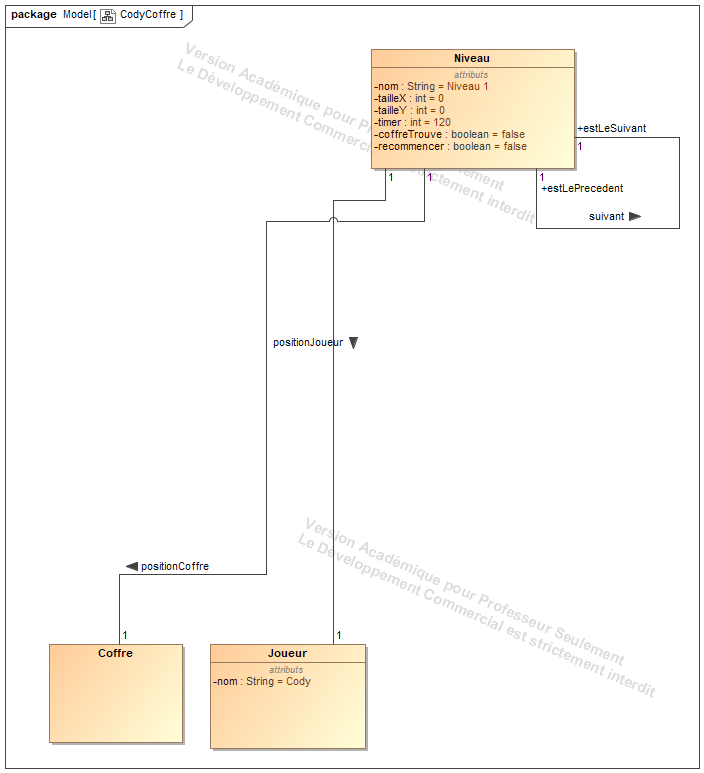
\includegraphics[width=400pt]{assets/CodyCoffre}
	\caption{Contrainte de Cody et du coffre}
	\label{fig:CodyCoffre}
\end{figure}

\newpage

La contrainte Ocl disant qu'un personnage ne peut se trouver sur un obstacle est exprimée comme suit:

\begin{lstlisting}[caption=Contrainte sur la position,captionpos=b,label={lst:positionobstacle},language=OCL]
context Niveau inv posobstacle:
    self.ElementNiveau->forall(p,o | 
        p.isOclTypeOf(Personnage) and 
        o.isOclTypeOf(Obstacle) and p.position.X <> o.position.X
             and p.position.Y <> o.position.Y)
\end{lstlisting}

La contrainte Ocl interdisant deux personnage de se trouver sur la même case est la suivante :

\begin{lstlisting}[caption=Contrainte sur l'interdiction de deux personnages sur la même case,captionpos=b,label={lst:interdiction},language=OCL]
context Niveau inv posperso:
    self.>ElementNiveau->forall(p1,p2 | 
        p1.isOclTypeOf(Personnage) 
        and p2.isOclTypeOf(Personnage) and p1 <> p2 implies 
            p1.position.X <> p2.position.X and
                 p1.position.Y <> p2.position.Y)
\end{lstlisting}

Le fait que le coffre doive se trouver sur une surface franchissable est caractérisé par la contrainte suivante:

\begin{lstlisting}[caption=Contrainte sur la position du coffre,captionpos=b,label={lst:poscoffre},language=OCL]
context Niveau inv poscoffre:
    self.ElementNiveau->forall(a,b | a.isOclTypeOf(Coffre)
         and b.isOclTypeOf(Sol) and a.position.X = b.position.X
             and a.position.Y = b.position.Y)
\end{lstlisting}

La contrainte exprimant le fait que chaque niveau comporte soit une paire de tunnels de téléportation de même couleur, soit un tunnel unique d'une couleur mais qui est initialement fermé s'exprime comme suit:

\begin{lstlisting}[caption=Contrainte sur les tunnels,captionpos=b,label={lst:tunnels},language=OCL]
context Niveau inv tunnel:
    (self.ElementNiveau->forall(t1,t2 | t1.isOclTypeOf(Tunnel) 
        and t2.isOclTypeOf(Tunnel) and t1.couleur = t2.couleur 
        and t1.isOpen = true and t2.isOpen = true) or 
        self.ElementNiveau->forall(t1| 
            t1.size() = 1 and t1.isOpen = false))
\end{lstlisting}

La propriété qu'un levier ne peut être présent que si il existe un tunnel de la même couleur est caractérisée comme suit:

\begin{lstlisting}[caption=Contrainte sur la présence d'un levier,captionpos=b,label={lst:présencelevier},language=OCL]
context Niveau inv levier:
    self.ElementNiveau->forall(l | l.isOclTypeOf(Levier) 
        and self.ElementNiveau->exists(t | t.isOclTypeOf(Tunnel)
        and l.couleur = t.couleur))
\end{lstlisting}

La contrainte exprimant qu'un obstacle ne peut se trouver que sur une surface franchissable est la quivante:

\begin{lstlisting}[caption=Contrainte sur les obstacles,captionpos=b,label={lst:posobstacles},language=OCL]
context Niveau inv obstacles:
    self.ElementNiveau->forall(a,b| a.isOclTypeOf(Obstacle) 
        and b.isOclTypeOf(Sol) and a.position.X == b.position.X 
            and a.position.Y == b.position.Y)
\end{lstlisting}